% Requer: tikz, calc
\begin{figure}[!htbp]
\centering
\resizebox{\textwidth}{!}{%
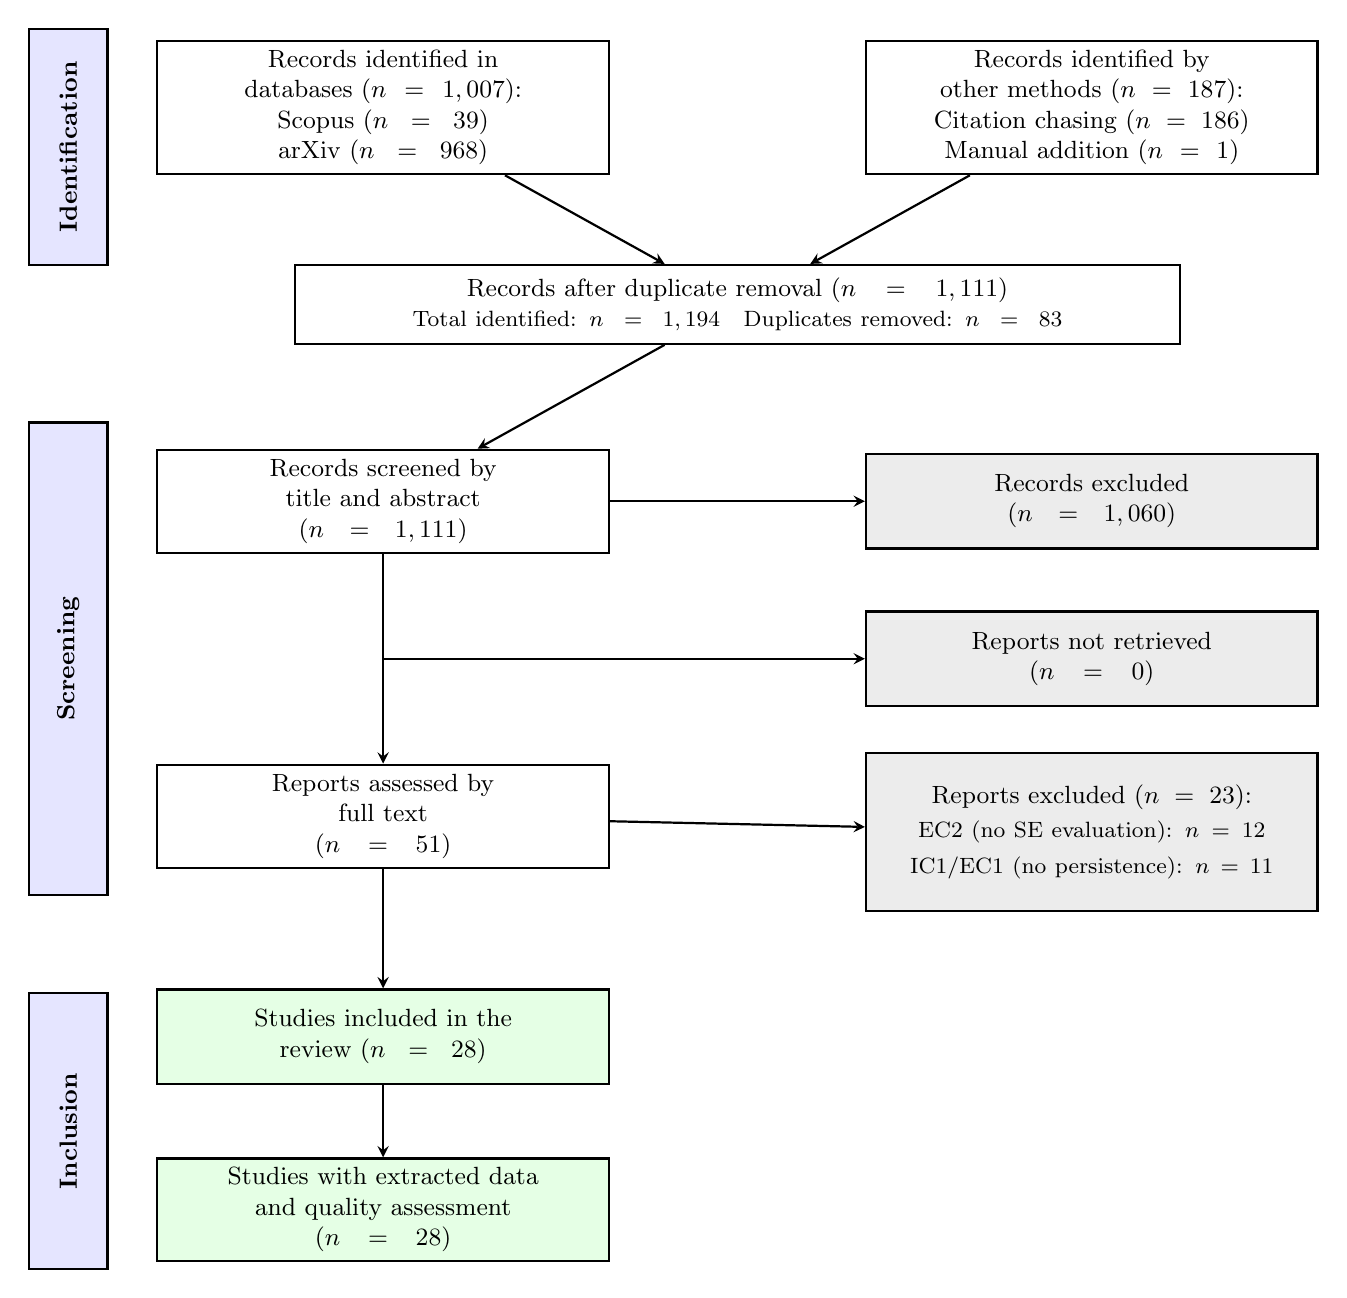
\begin{tikzpicture}[
  box/.style={rectangle, draw=black, thick, text width=5.5cm,
    minimum height=1.2cm, align=center, font=\small},
  boxwide/.style={rectangle, draw=black, thick, text width=11.0cm,
    minimum height=1.0cm, align=center, font=\small},
  boxgray/.style={rectangle, draw=black, thick, fill=gray!15,
    text width=5.5cm, minimum height=1.2cm, align=center, font=\small},
  phaselabel/.style={rectangle, draw=black, thick, fill=blue!10,
    minimum height=1.0cm, align=center,
    font=\small\bfseries, rotate=90, inner sep=3pt},
  arrow/.style={->, thick, >=stealth},
]
\node[phaselabel, minimum width=3.0cm] (l1) at (-2, -0.5)
  {Identification};
\node[phaselabel, minimum width=6.0cm] (l2) at (-2, -7.0)
  {Screening};
\node[phaselabel, minimum width=3.5cm] (l3) at (-2, -13.0)
  {Inclusion};

\node[box] (db) at (2, 0)
  {Records identified in\\databases ($n = 1,007$):\\
   Scopus ($n = 39$)\\arXiv ($n = 968$)};

\node[box] (other) at (11, 0)
  {Records identified by\\other methods ($n = 187$):\\
   Citation chasing ($n = 186$)\\
   Manual addition ($n = 1$)};

\node[boxwide] (dedup) at (6.5, -2.5)
  {Records after duplicate removal ($n = 1,111$)\\
   {\footnotesize Total identified: $n = 1,194$\quad
    Duplicates removed: $n = 83$}};

\draw[arrow] (db) -- (dedup);
\draw[arrow] (other) -- (dedup);

\node[box] (ta) at (2, -5.0)
  {Records screened by\\title and abstract\\($n = 1,111$)};

\node[boxgray] (ta_excl) at (11, -5.0)
  {Records excluded\\($n = 1,060$)};

\draw[arrow] (dedup) -- (ta);
\draw[arrow] (ta) -- (ta_excl);

\node[boxgray] (nr) at (11, -7.0)
  {Reports not retrieved\\($n = 0$)};

\node[box] (ft) at (2, -9.0)
  {Reports assessed by\\full text\\($n = 51$)};

\node[boxgray, minimum height=2.0cm] (ft_excl) at (11, -9.2)
  {Reports excluded ($n = 23$):\\[3pt]
   {\footnotesize
   EC2 (no SE evaluation): $n = 12$\\[2pt]
   IC1/EC1 (no persistence): $n = 11$}};

\draw[arrow] (ta) -- (ft);
\draw[arrow] (2, -7.0) -- (nr.west);
\draw[arrow] (ft) -- (ft_excl);

\node[box, fill=green!10] (incl) at (2, -11.8)
  {Studies included in the\\review ($n = 28$)};

\draw[arrow] (ft) -- (incl);

\node[box, fill=green!10] (qual) at (2, -14.0)
  {Studies with extracted data\\and quality assessment\\($n = 28$)};

\draw[arrow] (incl) -- (qual);

\end{tikzpicture}%
}
\caption{PRISMA 2020 flow diagram for this systematic review.
Adapted from \citet{page2021prisma}.}
\label{fig:prisma-flow}
\end{figure}
